\begin{frame}
	\frametitle{Neutronics Verification}
		\begin{columns}
			\column{5cm}
				\textbf{Serpent Input Parameters}
					\begin{itemize}
						\item 200,000 neutrons per cycle
						\item 50 inactive, 500 active cycles
						\item JEFF-3.1.2 nuclear data library
						\item Six neutron energy groups, eight \gls{DNP} groups
						\item Temperatures defined from 900 K to 1200 K at 50 K
						intervals
					\end{itemize}
			\column{5cm}
				\begin{figure}
					\centering
					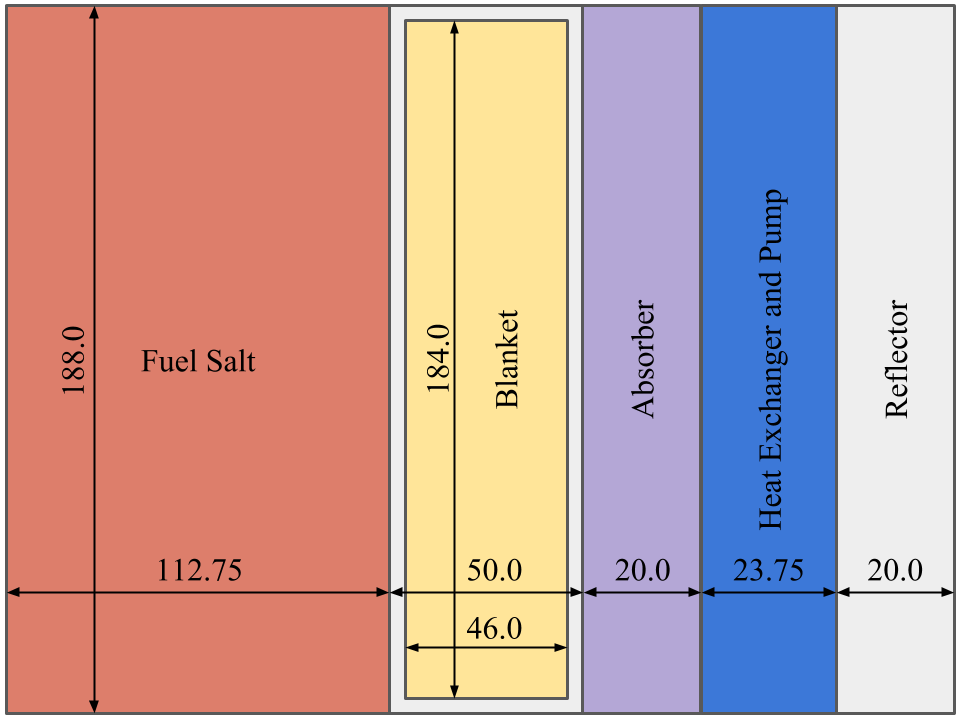
\includegraphics[width=\textwidth]
					{../paper/figures/reference}
					\caption{2D axisymmetric model used in Serpent. Derived from
					the \gls{MSFR} reference model
					\cite{fiorina_modelling_2014}.}
					\label{fig:reference}
				\end{figure}
		\end{columns}
\end{frame}

\begin{frame}
	\frametitle{Neutronics Verification}
		\textbf{Fuel Composition Data}
			\begin{itemize}
				\item Depletion calculations performed by Rykhlevskii et
				al. \cite{rykhlevskii_fuel_2019}
				\item 60-year depletion calculation on SCALE/TRITON
				using a unit cell representation of the \gls{MSFR} (and
				three other fast-spectrum \glspl{MSR}
				\item U/Th breeder reprocessing scheme
				\item Compositions:
				\begin{itemize}
					\item Start-up: 77.5\% LiF - 19.9\% ThF$_4$
					- 2.6\% UF$_4$
					\item Early-life: 300 days after start-up
					\item Equilibrium: ~43 years after start-up
					($<$3\% change in TRU vector between depletion
					time-steps)
				\end{itemize}
			\end{itemize}
\end{frame}

\begin{frame}
	\frametitle{Neutronics Verification}
	\begin{columns}
		\column{5cm}
		\textbf{Moltres Simulation Details}
		\begin{itemize}
			\item Adaptive backward Euler time-stepper
			\item Six neutron groups, eight \gls{DNP} groups
			\item Vacuum neutron boundary condition on outer surfaces
			\item Uniform upward flow of 1.125 m s$^{-1}$
			\item Flow/decay of \glspl{DNP} and heat removal in the outer loop
			is simulated on a simplified 1D geometry separate from active core
			region
			\item Fixed heat removal rate to secondary loop system
		\end{itemize}
		\column{5cm}
		\begin{figure}
			\centering
			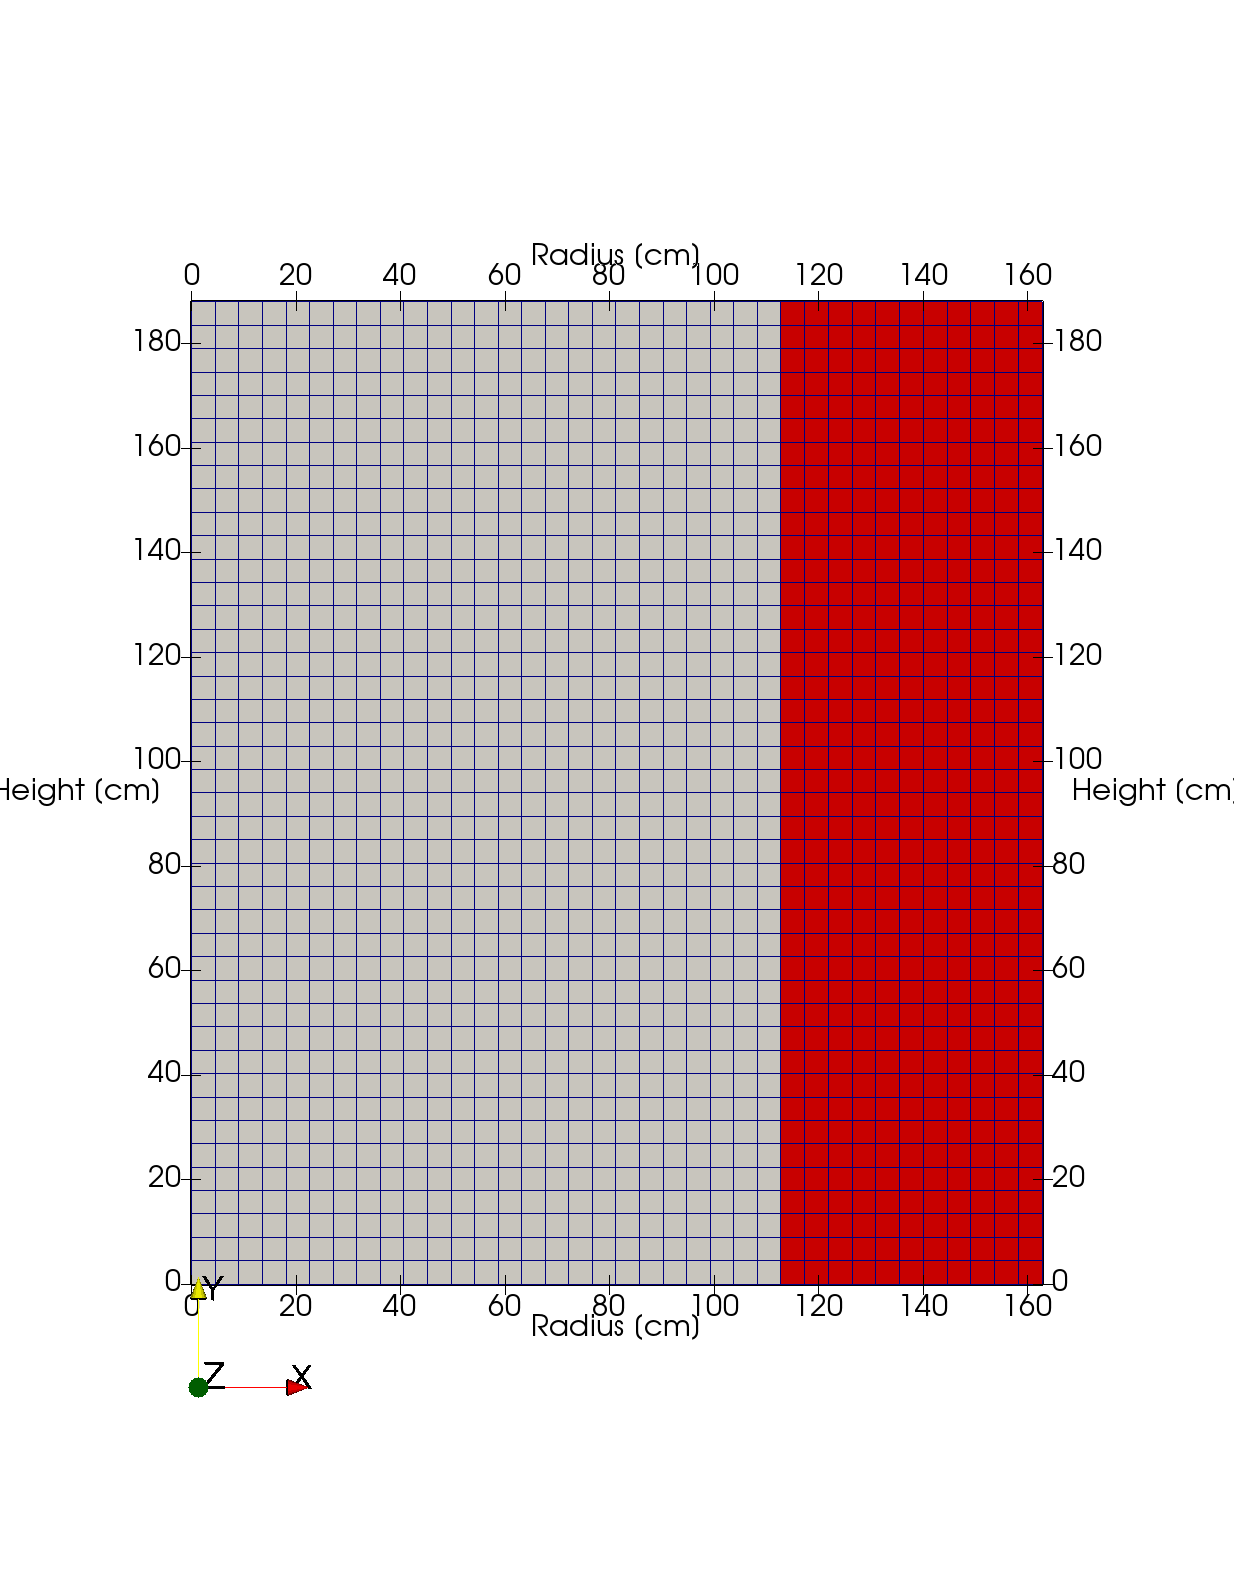
\includegraphics[width=.8\textwidth]{../paper/figures/mesh}
			\caption{Mesh of the 2D axisymmetric model used in Moltres. The
			grey and red regions represent the fuel and blanket salt
			respectively.}
			\label{fig:mesh}
		\end{figure}
	\end{columns}
\end{frame}

\begin{frame}
	\frametitle{Neutronics Verification}
		\textbf{Results}
			\begin{figure}
				\centering
				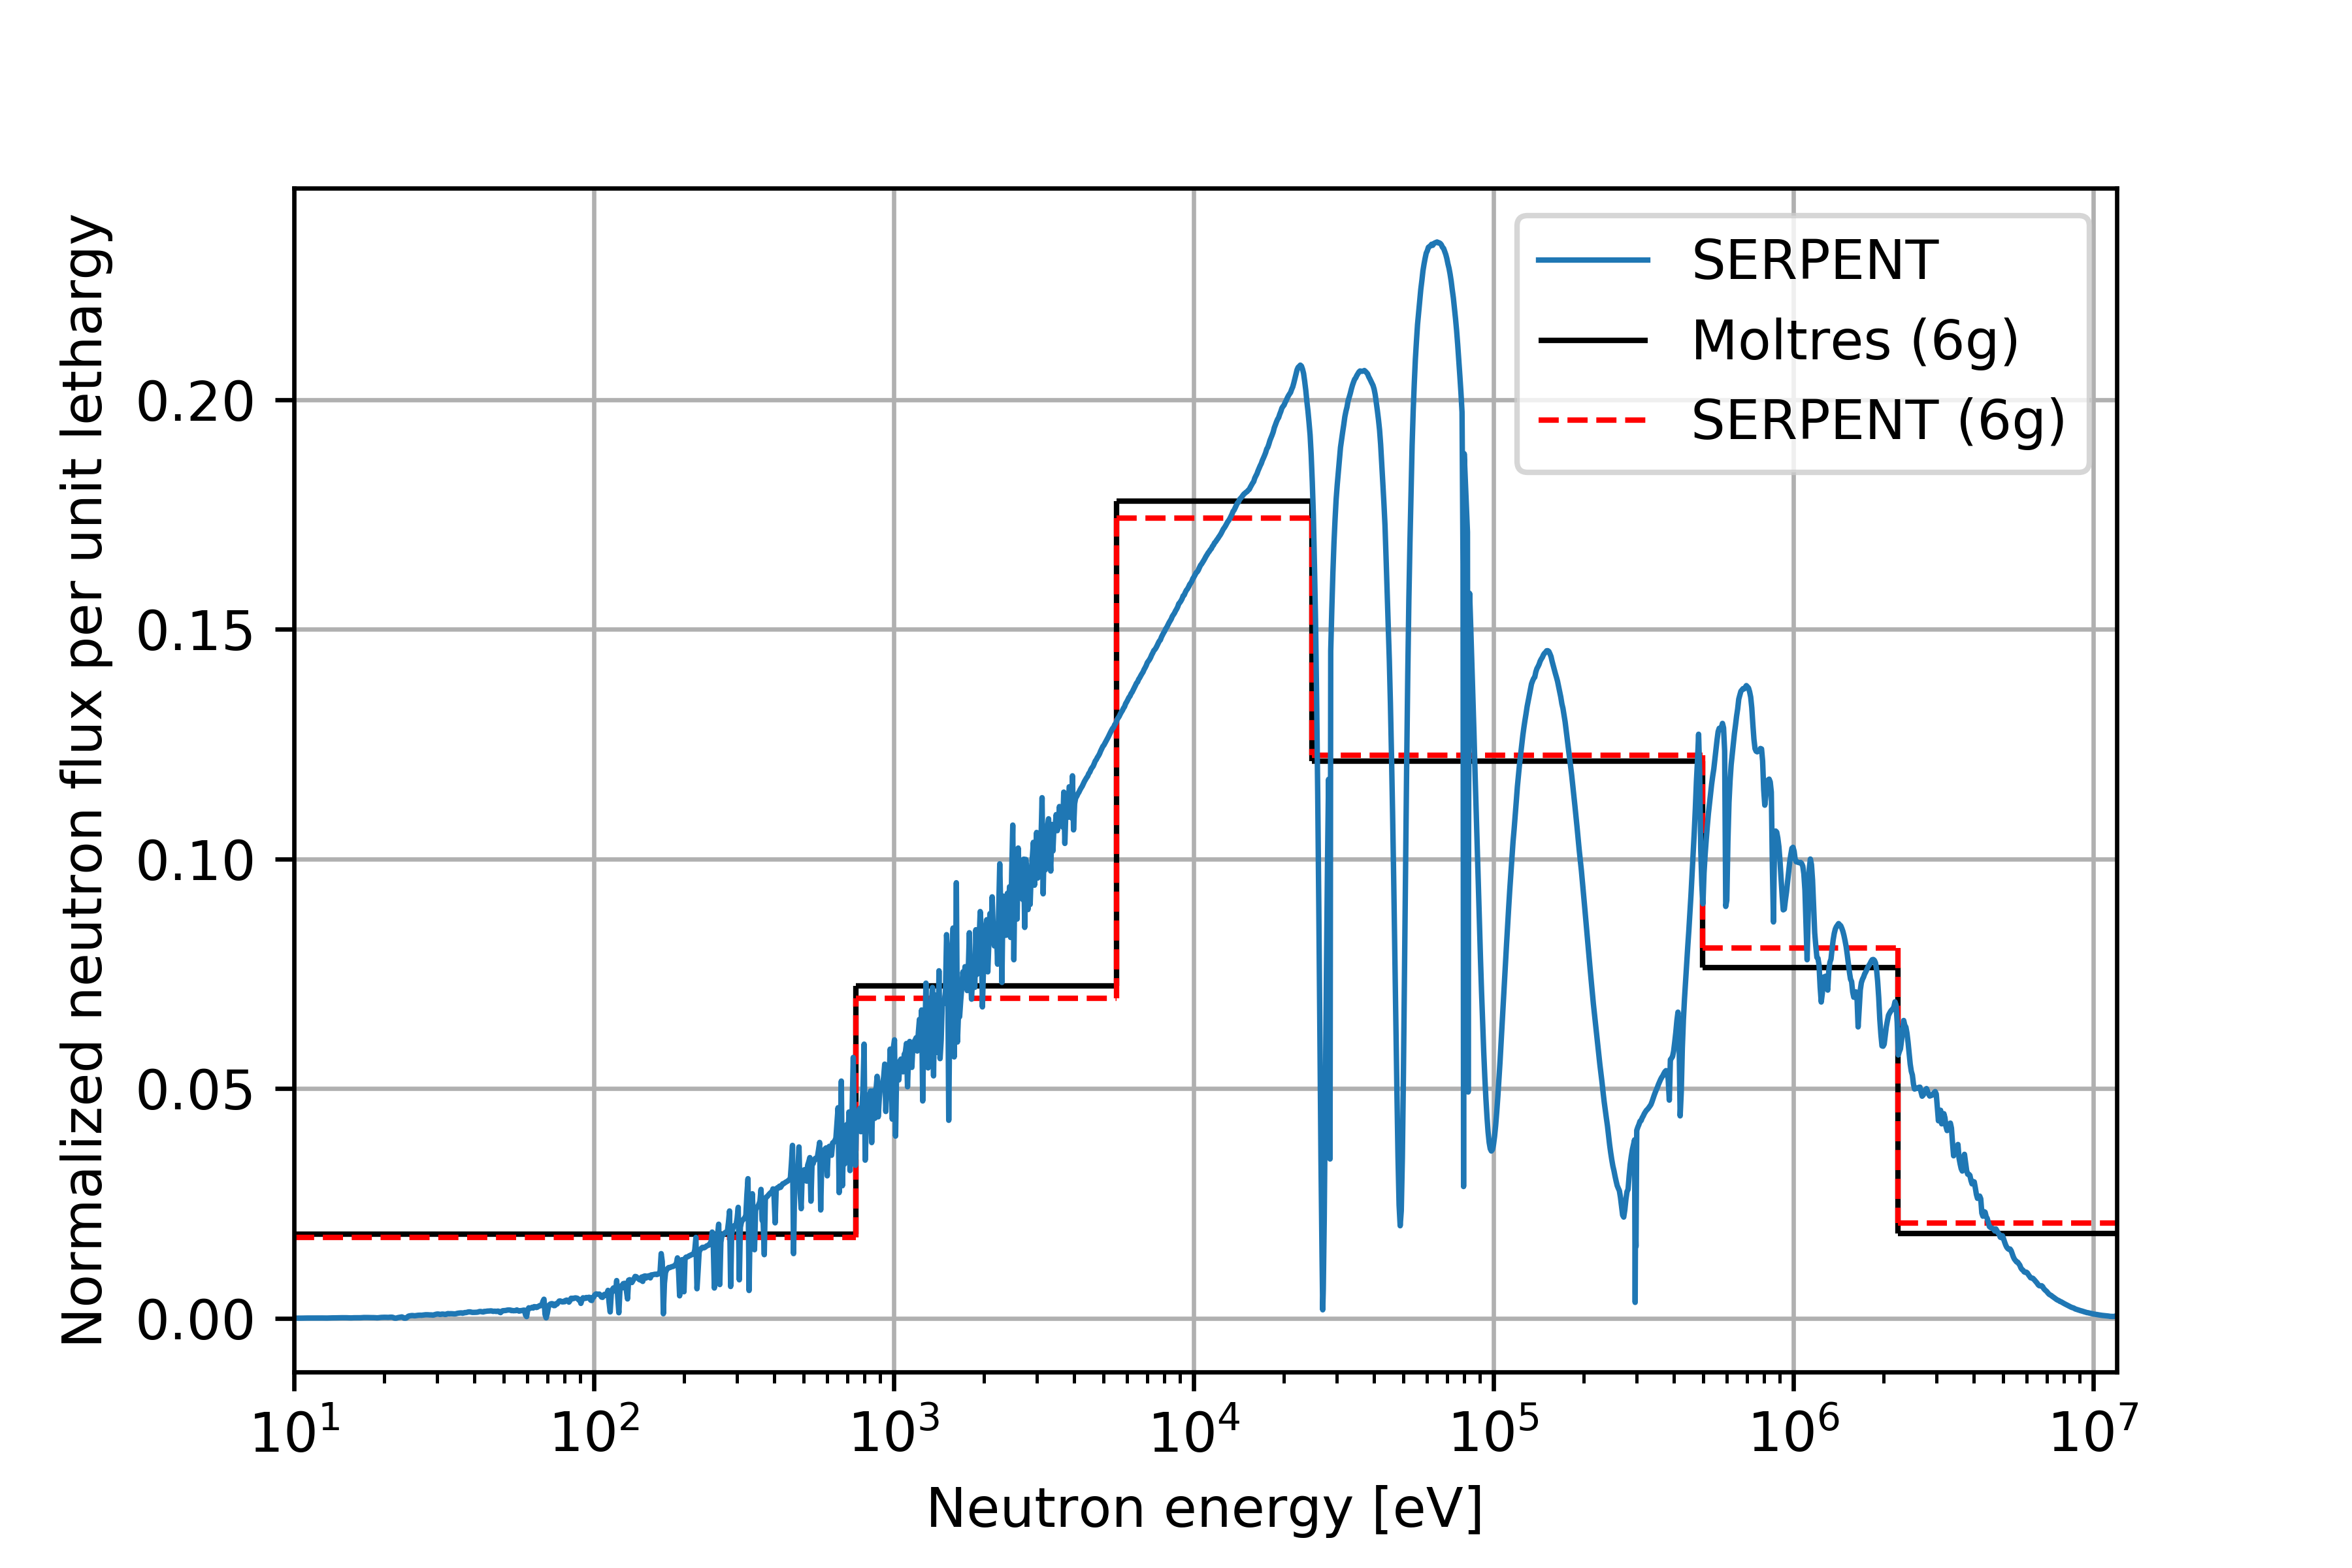
\includegraphics[width=.8\textwidth]{../paper/figures/nt-spec}
				\caption{Fine-group and six-group neutron flux distributions
				from Serpent and Moltres (start-up composition without \gls{DNP}
				drift).}
				\label{fig:ntspec}
			\end{figure}
\end{frame}
